%%%%%%%%%%%%%%%%%%%%%%%%%%%%%%%%%%%%%%%
% Wenneker Resume/CV
% LaTeX Template
% Version 1.1 (19/6/2016)
%
% This template has been downloaded from:
% http://www.LaTeXTemplates.com
%
% Original author:
% Frits Wenneker (http://www.howtotex.com) with extensive modifications by 
% Vel (vel@LaTeXTemplates.com) and Jerzy Tomes (visual changes, lualatex, etc)
% 
% License:
% CC BY-NC-SA 3.0 (http://creativecommons.org/licenses/by-nc-sa/3.0/
%
%%%%%%%%%%%%%%%%%%%%%%%%%%%%%%%%%%%%%%

%----------------------------------------------------------------------------------------
%	PACKAGES AND OTHER DOCUMENT CONFIGURATIONS
%----------------------------------------------------------------------------------------

\documentclass[a4paper,12pt]{memoir} % Font and paper size
\hyphenation{capabilities, Postman}
%%%%%%%%%%%%%%%%%%%%%%%%%%%%%%%%%%%%%%%%%
% Wenneker Resume/CV
% Structure Specification File
% Version 1.1 (19/6/2016)
%
% This file has been downloaded from:
% http://www.LaTeXTemplates.com
%
% Original author:
% Frits Wenneker (http://www.howtotex.com) with extensive modifications by 
% Vel (vel@latextemplates.com) and Jerzy Tomes
%
% License:
% CC BY-NC-SA 3.0 (http://creativecommons.org/licenses/by-nc-sa/3.0/)
%
%%%%%%%%%%%%%%%%%%%%%%%%%%%%%%%%%%%%%%%%%

%----------------------------------------------------------------------------------------
%	PACKAGES AND OTHER DOCUMENT CONFIGURATIONS
%----------------------------------------------------------------------------------------

\usepackage{fontspec} % fonty systemowe
\setmainfont{Ubuntu}
\setmonofont{Ubuntu Mono}
\usepackage[utf8]{inputenc} % Required for inputting international characters
% \usepackage[T1]{fontenc} % Output font encoding for international characters

\usepackage[top=1cm,left=1cm,right=1cm,bottom=1cm]{geometry} % Modify margins

\usepackage{graphicx} % Required for figures

\usepackage{flowfram} % Required for the multi-column layout
\usepackage{multicol}

\usepackage{url} % URLs
\usepackage{hyperref} % make them clickable

\usepackage[usenames,dvipsnames]{xcolor} % Required for custom colours

\usepackage{tikz} % Required for the horizontal rule
\usetikzlibrary{patterns}

\usepackage{enumitem} % Required for modifying lists
\setlist{noitemsep,nolistsep} % Remove spacing within and around lists

\setlength{\columnsep}{\baselineskip} % Set the spacing between columns

% Define the left frame (sidebar)
\newflowframe{0.25\textwidth}{\textheight}{0pt}{0pt}[left]
\newlength{\LeftMainSep}
\setlength{\LeftMainSep}{0.25\textwidth}
\addtolength{\LeftMainSep}{1\columnsep}
 
% Small static frame for the vertical line
\newstaticframe{1.5pt}{\textheight}{\LeftMainSep}{0pt}
 
% Content of the static frame with the vertical line
\begin{staticcontents}{1}
\hfill
\tikz{\draw[dash pattern=on 1pt off 1pt on 2pt off 1pt on 2pt off 1pt on 2pt
        off 2pt on 1pt off 2pt on 1pt off 1pt on 2pt off 1pt on 1pt off 2pt on
        2pt off 1pt on 2pt off 1pt on 1pt off 1pt on 1pt off 2pt on 2pt off 1pt
        on 1pt off 1pt on 2pt off 1pt on 2pt off 3pt, color=NavyBlue, line
        width=1.5pt,yshift=0](0,0) -- (0,\textheight);} % sorry not sorry.
        % replace with something sensible before reuse
\hfill\mbox{}
\end{staticcontents}
 
% Define the right frame (main body)
\addtolength{\LeftMainSep}{1.5pt}
\addtolength{\LeftMainSep}{1\columnsep}
\newflowframe{0.65\textwidth}{\textheight}{\LeftMainSep}{0pt}[main01]

\pagestyle{empty} % Disable all page numbering

\setlength{\parindent}{0pt} % Stop paragraph indentation

%----------------------------------------------------------------------------------------
%	NEW COMMANDS
%----------------------------------------------------------------------------------------

\newcommand{\userinformation}[1]{\renewcommand{\userinformation}{#1}} % Define a new command for the CV user's information that goes into the left column

\newcommand{\cvheading}[1]{{\Huge\bfseries\color{NavyBlue} #1} \par\vspace{.6\baselineskip}} % New command for the CV heading
\newcommand{\cvsubheading}[1]{{\Large\bfseries #1} \bigbreak} % New command for the CV subheading

\newcommand{\Sep}{\vspace{1em}} % New command for the spacing between headings
\newcommand{\SmallSep}{\vspace{0.5em}} % New command for the spacing within headings

\newcommand{\aboutme}[2]{ % New command for the about me section
\textbf{\color{NavyBlue} #1}~~#2\par\Sep
}
	
\newcommand{\CVSection}[1]{ % New command for the headings within sections
{\Large\textbf{#1}}\par
\SmallSep % Used for spacing
}

\newcommand{\CVItem}[2]{ % New command for the item descriptions
\textbf{\color{NavyBlue} #1}\par
#2
\SmallSep % Used for spacing
}

\newcommand{\bluebullet}{\textcolor{NavyBlue}{$\circ$}~~} % New command for the blue bullets
 % Include the file specifying document layout and packages

%----------------------------------------------------------------------------------------
%	NAME AND CONTACT INFORMATION 
%----------------------------------------------------------------------------------------

\userinformation{ % Set the content that goes into the sidebar of each page
\begin{flushright}
% Comment out this figure block if you don't want a photo
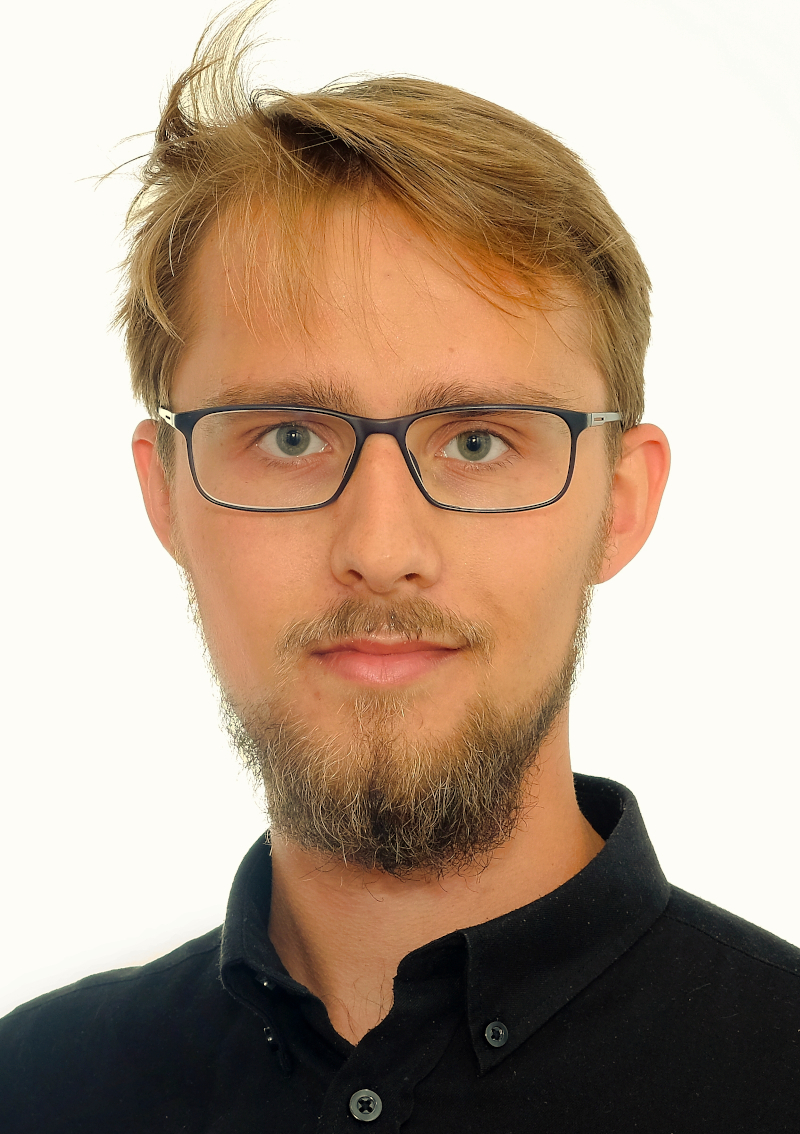
\includegraphics[width=0.7\columnwidth]{photo.jpg}\\[\baselineskip] % Your photo
\small % Smaller font size
Jerzy Tomes \\ % Your name
\url{jerzy.tomes@gmail.com} \\ % Your email address
505 845 539 \\ % Your phone number
\Sep
\url{linkedin.com/in/jerzy-tomes}
\Sep\\
automation examples:
\url{github.com/Jerzy-Tomes}
\Sep % Some whitespace
% \textbf{Address} \\
% 123 Broadway \\ % Address 1
% City, State 12345 \\ % Address 2
% Country \\ % Address 3
\vfill % Whitespace under this block to push it up under the photo
\end{flushright}
}

%----------------------------------------------------------------------------------------

\begin{document}

\userinformation % Print your information in the left column

\framebreak % End of the first column

%----------------------------------------------------------------------------------------
%	HEADING
%----------------------------------------------------------------------------------------

\cvheading{Jerzy Tomes} % Large heading - your name

\cvsubheading{Software QA Engineer Candidate} % Subheading - your occupation/specialization

%----------------------------------------------------------------------------------------
%	ABOUT ME
%----------------------------------------------------------------------------------------

\aboutme{About Me}{Recent graduate of MSc studies in Biomedical Engineering,
with specialty in Medical Informatics, at Wroclaw University of Science and
Technology. My master thesis concerned use of Machine Learning in diagnostics.
Following my decision to become a tester, I obtained an ISTQB
certificate and started learning testing and automation tools. 
Currently, I'm gaining experience with crowdtesting sites.

I am searching for a Junior or Intern position in Software QA sector, which
will allow me to start IT career and build up experience.}

%----------------------------------------------------------------------------------------
%	EDUCATION
%----------------------------------------------------------------------------------------

\CVSection{Education and Certification}

%------------------------------------------------
\CVItem{2021, ISTQB Foundation Level certificate}{Acquired after preparation
course with testuj.pl}

%------------------------------------------------

\CVItem{2019 - 2020, Wroclaw University of Science and Technology}{MSc in
Biomedical Engineering, specialty: Medical Informatics}

%------------------------------------------------


\CVItem{2015 - 2019, Wroclaw University of Science and Technology}{BSc in
Biomedical Engineering, specialty: Medical Informatics}


%------------------------------------------------

\Sep % Extra whitespace after the end of a major section

%----------------------------------------------------------------------------------------
%	EXPERIENCE
%----------------------------------------------------------------------------------------

\CVSection{Experience}

%------------------------------------------------

\CVItem{2015 - 2020: \textit{miscellaneous temporary jobs}}

\CVItem{2018, 2019: \textit{election commission member}}

\CVItem{2021: \textit{crowdtesting platforms: mainly utest.com and
testerwork.com}}

%------------------------------------------------

% \CVItem{Jan 2008 - Oct 2012, \textit{Computer Repair Specialist}, Buy More}{Worked in the Nerd Herd and helped to solve computer problems by asking customers to turn their computers off and on again.}

%------------------------------------------------

\Sep % Extra whitespace after the end of a major section

%----------------------------------------------------------------------------------------
%	COMMUNICATION SKILLS
%----------------------------------------------------------------------------------------
%
%\CVSection{Communication Skills}
%
%%------------------------------------------------
%
%\CVItem{2015, \textit{Oral Presentation}, California Business Conference}{Presented research I conducted for my Masters of Engineering degree.}
%
%%------------------------------------------------
%
%\CVItem{2014, \textit{Poster}, Annual Business Conference (Oregon)}{As part of the course work for BUS320, I created a poster analyzing several local businesses and presented this at a conference.}
%
%%------------------------------------------------
%
%\Sep % Extra whitespace after the end of a major section

%----------------------------------------------------------------------------------------
%	SKILLS
%----------------------------------------------------------------------------------------

\CVSection{Work Skills}

%------------------------------------------------
%------------------------------------------------

\CVItem{Skills}
{\begin{itemize}
    \item[\bluebullet] Theory of testing and software development process
%    \item[\bluebullet] Experience with office suites (Libre and MS) and \LaTeX 
    \item[\bluebullet] Git, Kanban Boards, Jira basics and teamwork capabilities
    \item[\bluebullet] REST and SOAP API testing in SOAP UI and Postman
    \item[\bluebullet] Automation with Selenium and Cypress.io, BDD testing
            (Gherkin)
    \item[\bluebullet] Python, shell, SQL, Java, Matlab
    \item[\bluebullet] Meticulousness and test to break attitude
    \item[\bluebullet] Inclination to learn and experience new things
\end{itemize}}
%------------------------------------------------
%
%\CVItem{Programming Languages}
%{\parbox{0.5\textwidth}{
%        \begin{multicols}{3}
%        \begin{itemize}
%                \item[\bluebullet] Python
%                \item[\bluebullet] Shell
%                \item[\bluebullet] SQL
%                \item[\bluebullet] Java 
%                \item[\bluebullet] Matlab
%        \end{itemize}
%\end{multicols}}}
%
%
\CVItem{Languages} 
{Polish (native), English (advanced), learning or re-learning: French, German,
Russian (elementary), Arabic (beginner)}
% {\begin{multicols}{2}
%         \begin{itemize}
%                 \item[\bluebullet] English (advanced) 
%                 \item[\bluebullet] French (elementary)
%                 \item[\bluebullet] Russian (elementary) 
%                 \item[\bluebullet] Arabic (beginner)
%                 \item[\bluebullet] Polish (native)
%         \end{itemize}
%         \end{multicols}}
% 
\Sep % Extra whitespace after the end of a major section

%----------------------------------------------------------------------------------------
%	NEW PAGE DELIMITER
%	Place this block wherever you would like the content of your CV to go onto the next page
%----------------------------------------------------------------------------------------
%
%\clearpage % Start a new page
%
%\userinformation % Print your information in the left column
%
%\framebreak % End of the first column
%
%----------------------------------------------------------------------------------------
%	AWARDS
%----------------------------------------------------------------------------------------

%\CVSection{Awards}
%
%------------------------------------------------
%
%\CVItem{2010, \textit{Postgraduate Scholarship}, Cornell University}{Awarded to the top student in their final year of a Bachelors degree.}
%
%------------------------------------------------
%
%\Sep  Extra whitespace after the end of a major section
%
%----------------------------------------------------------------------------------------
%	INTERESTS
%----------------------------------------------------------------------------------------

\CVSection{Interests}

%------------------------------------------------

\CVItem{Professional}{Software QA, Machine Learning}

%------------------------------------------------

\CVItem{Personal}{Language learning, PICO-8, hiking, running}

%------------------------------------------------

\Sep % Extra whitespace after the end of a major section

%----------------------------------------------------------------------------------------

\end{document}
